\part{\RU{Поиск в коде того что нужно}\EN{Finding important/interesting stuff in the code}}

\RU{Современное ПО, в общем-то, минимализмом не отличается.}
\EN{Minimalism it is not a prominent feature of modern software.}

\index{\Cpp!STL}
\RU{Но не потому, что программисты слишком много пишут, 
а потому что к исполняемым файлам обыкновенно прикомпилируют все подряд библиотеки. 
Если бы все вспомогательные библиотеки всегда выносили во внешние DLL, мир был бы иным.
(Еще одна причина для Си++ ~--- STL и прочие библиотеки шаблонов.)}
\EN{But not because the programmers are writing a lot, but because a lot of libraries are commonly linked statically
to executable files.
If all external libraries were shifted into an external DLL files, the world would be different.
(Another reason for C++ are the STL and other template libraries.)}

\newcommand{\FOOTNOTEBOOST}{\footnote{\url{http://go.yurichev.com/17036}}}
\newcommand{\FOOTNOTELIBPNG}{\footnote{\url{http://go.yurichev.com/17037}}}

\RU{Таким образом, очень полезно сразу понимать, какая функция из стандартной библиотеки или 
более-менее известной (как Boost\FOOTNOTEBOOST, libpng\FOOTNOTELIBPNG), 
а какая ~--- имеет отношение к тому что мы пытаемся найти в коде.}
\EN{Thus, it is very important to determine the origin of a function, if it is from standard library or 
well-known library (like Boost\FOOTNOTEBOOST, libpng\FOOTNOTELIBPNG),
or if it is related to what we are trying to find in the code.}

\RU{Переписывать весь код на \CCpp, чтобы разобраться в нем, безусловно, не имеет никакого смысла.}
\EN{It is just absurd to rewrite all code in \CCpp to find what we're looking for.}

\RU{Одна из важных задач reverse engineer-а это быстрый поиск в коде того что собственно его интересует.}
\EN{One of the primary tasks of a reverse engineer is to find quickly the code he/she needs.}

\index{\GrepUsage}
\RU{Дизассемблер \IDA позволяет делать поиск как минимум строк, последовательностей байт, констант.
Можно даже сделать экспорт кода в текстовый файл .lst или .asm и затем натравить на него \TT{grep}, \TT{awk}, и т.д.}
\EN{The \IDA disassembler allow us to search among text strings, byte sequences and constants.
It is even possible to export the code to .lst or .asm text files and then use \TT{grep}, \TT{awk}, etc.}

\RU{Когда вы пытаетесь понять, что делает тот или иной код, это запросто может быть какая-то 
опенсорсная библиотека вроде libpng. Поэтому, когда находите константы, или текстовые строки, которые 
выглядят явно знакомыми, всегда полезно их \IT{погуглить}.
А если вы найдете искомый опенсорсный проект где это используется, 
то тогда будет достаточно будет просто сравнить вашу функцию с ней. 
Это решит часть проблем.}
\EN{When you try to understand what some code is doing, this easily could be some open-source library like libpng.
So when you see some constants or text strings which look familiar, it is always worth to \IT{google} them.
And if you find the opensource project where they are used, 
then it will be enough just to compare the functions.
It may solve some part of the problem.}

\RU{К примеру, если программа использует какие-то XML-файлы, первым шагом может быть
установление, какая именно XML-библиотека для этого используется, ведь часто используется какая-то
стандартная (или очень известная) вместо самодельной.}
\EN{For example, if a program uses XML files, the first step may be determining which
XML library is used for processing, since the standard (or well-known) libraries are usually used
instead of self-made one.}

\index{SAP}
\index{Windows!PDB}
\RU{К примеру, однажды я пытался разобраться как происходит компрессия/декомпрессия сетевых пакетов в SAP 6.0. 
Это очень большая программа, но к ней идет подробный .\gls{PDB}-файл с отладочной информацией, и это очень удобно. 
Я в конце концов пришел к тому что одна из функций декомпрессирующая пакеты называется CsDecomprLZC(). 
Не сильно раздумывая, я решил погуглить и оказалось, что функция с таким же названием имеется в MaxDB
(это опен-сорсный проект SAP)\footnote{Больше об этом в соответствующей секции~(\myref{sec:SAPGUI})}.}
\EN{For example, once I tried to understand how the compression/decompression of network packets worked in SAP 6.0. 
It is a huge software, but a detailed .\gls{PDB} with debugging information is present, 
and that is convenient.
I finally came to the idea that one of the functions, that was called CsDecomprLZC, was doing the decompression of network packets.
Immediately I tried to google its name and I quickly found the function was used in MaxDB
(it is an open-source SAP project)\footnote{More about it in relevant section~(\myref{sec:SAPGUI})}.}

\url{http://www.google.com/search?q=CsDecomprLZC}

\RU{Каково же было мое удивление, когда оказалось, что в MaxDB используется точно такой же алгоритм, 
скорее всего, с таким же исходником.}
\EN{Astoundingly, MaxDB and SAP 6.0 software shared likewise code for the compression/decompression of network packets.}

\chapter{\RU{Идентификация исполняемых файлов}\EN{Identification of executable files}}

\section{Microsoft Visual C++}

\RU{Версии MSVC и DLL которые могут быть импортированы}\EN{MSVC versions and DLLs which may be imported}:

\begin{center}
\begin{tabular}{ | l | l | l | l | l | }
\hline
\cellcolor{blue!25} \RU{Маркетинговая версия}\EN{Marketing version} & 
\cellcolor{blue!25} \RU{Внутренняя версия}\EN{Internal version} & 
\cellcolor{blue!25} \RU{Версия }CL.EXE\EN{ version} &
\cellcolor{blue!25} \RU{Импортируемые DLL}\EN{DLLs may be imported} &
\cellcolor{blue!25} \RU{Дата выхода}\EN{Release date} \\
\hline
% 4.0, April 1995
% 97 & 5.0 & February 1997
6		&  6.0 & 12.00 & msvcrt.dll, msvcp60.dll    & June 1998 \\
\hline
.NET (2002)	&  7.0 & 13.00 & msvcr70.dll, msvcp70.dll   & February 13, 2002 \\
\hline
.NET 2003	&  7.1 & 13.10 & msvcr71.dll, msvcp71.dll   & April 24, 2003 \\
\hline
2005		&  8.0 & 14.00 & msvcr80.dll, msvcp80.dll   & November 7, 2005 \\
\hline
2008		&  9.0 & 15.00 & msvcr90.dll, msvcp90.dll   & November 19, 2007 \\
\hline
2010		& 10.0 & 16.00 & msvcr100.dll, msvcp100.dll & April 12, 2010 \\
\hline
2012		& 11.0 & 17.00 & msvcr110.dll, msvcp110.dll & September 12, 2012 \\
\hline
2013		& 12.0 & 18.00 & msvcr120.dll, msvcp120.dll & October 17, 2013 \\
\hline
\end{tabular}
\end{center}

msvcp*.dll \RU{содержит ф-ции связанные с Си++, так что если она импортируется, скорее всего, 
вы имеете дело с программой на Си++}\EN{contain C++-related functions, so, if it is imported, 
this is probably C++ program}.

\subsection{Name mangling}

\RU{Имена обычно начинаются с символа}\EN{Names are usually started with} \TT{?}\EN{ symbol}.

\RU{О}\EN{Read more about MSVC} \gls{name mangling} \RU{в MSVC читайте также здесь}\EN{here}: \ref{namemangling}.

\section{GCC}
\index{GCC}

\RU{Кроме компиляторов под *NIX, GCC имеется так же и для win32-окружения: в виде}
\EN{Aside from *NIX targets, GCC is also present in win32 environment: in form of} Cygwin \AndENRU MinGW.

\subsection{Name mangling}

\RU{Имена обычно начинаются с символов}\EN{Names are usually started with} \TT{\_Z}\EN{ symbols}.

\RU{О}\EN{Read more about GCC} \gls{name mangling} \RU{в GCC читайте также здесь}\EN{here}: \ref{namemangling}.

\subsection{Cygwin}
\index{Cygwin}

cygwin1.dll \RU{часто импортируется}\EN{is often imported}.

\subsection{MinGW}
\index{MinGW}

msvcrt.dll \RU{может импортироваться}\EN{may be imported}.

\section{Intel FORTRAN}
\index{FORTRAN}

libifcoremd.dll, libifportmd.dll \AndENRU libiomp5md.dll (\RU{поддрежка }OpenMP\EN{ support}) 
\RU{могут импортироваться}\EN{may be imported}.

\RU{В }libifcoremd.dll \RU{много ф-ций с префиксом}\EN{has a lot of functions prefixed with} 
\TT{for\_}, \RU{что значит}\EN{meaning} FORTRAN.

\section{Watcom, OpenWatcom}
\index{Watcom}
\index{OpenWatcom}

\subsection{Name mangling}

\RU{Имена обычно начинаются с символа}\EN{Names are usually started with} \TT{W}\EN{ symbol}.

\RU{Например, так кодируется метод ``method'' класса ``class'' не имеющий аргументов и возвращающий \Tvoid}
\EN{For example, that is how method named ``method'' of the class ``class'' not having arguments and returning
\Tvoid is encoded to}:

\begin{lstlisting}
W?method$_class$n__v
\end{lstlisting}

\section{Borland}
\index{Borland Delphi}
\index{Borland C++Builder}

\RU{Вот пример \gls{name mangling} в Borland Delphi и C++Builder}
\EN{Here is an example of Borland Delphi and C++Builder \gls{name mangling}}:

\lstinputlisting{digging_into_code/identification/borland_mangling.txt}

\RU{Имена всегда начинаются с символа}\EN{Names are always started with} \TT{@} 
\RU{затем следует имя класса, имя метода
и закодированные типы аргументов}\EN{symbol, then class name came, method name, and encoded method argument types}.

\RU{Эти имена могут присутствовать с импортах .exe, экспортах .dll, отладочной информации, и т.д}
\EN{These names can be in .exe imports, .dll exports, debug data, etc}.

Borland Visual Component Libraries (VCL) \RU{находятся в файлах .bpl вместо .dll, например}
\EN{are stored in .bpl files instead of .dll ones, for example}, vcl50.dll, rtl60.dll.

\RU{Другие DLL которые могут импортироваться}\EN{Other DLL might be imported}: BORLNDMM.DLL.

\subsection{Delphi}

\RU{Почти все исполняемые файлы имеют текстовую строку}\EN{Almost all Delphi executables has} ``Boolean'' 
\RU{в самом начале сегмента кода, среди остальных имен типов}
\EN{text string at the very beginning of code segment, along with other type names}.

\RU{Вот очень характерное для Delphi начало сегмента \TT{.text}, 
этот блок следует сразу за заголовком win32 PE-файла}
\EN{This is a very typical beginning of \TT{.text} 
segment of a Delphi program, this block came right after win32 PE file header}:

\lstinputlisting{digging_into_code/identification/delphi.txt}

\section{\RU{Другие известные DLL}\EN{Other known DLLs}}

\begin{itemize}
\index{OpenMP}
\item vcomp*.dll\EMDASH{}\RU{Реализация OpenMP от Microsoft}\EN{Microsoft implementation of OpenMP}.
\end{itemize}


% binary files might be also here
\chapter{\RU{Связь с внешним миром}\EN{Communication with the outer world} (win32)}

\RU{Иногда, чтобы понять что делает та или иная функция, можно её не разбирать, а просто посмотреть на её входы и выходы.}%
\EN{Sometimes it's enough to observe some function's inputs and outputs in order to understand what it does.}
\RU{Так можно сэкономить время}\EN{That way you can save time}.

\RU{Обращения к файлам и реестру}\EN{Files and registry access}: 
\RU{для самого простого анализа может помочь утилита}%
\EN{for the very basic analysis, } Process Monitor\footnote{\url{http://go.yurichev.com/17301}}
\RU{от}\EN{utility from} SysInternals\EN{ can help}.

\RU{Для анализа обращения программы к сети, может помочь}%
\EN{For the basic analysis of network accesses,} Wireshark\footnote{\url{http://go.yurichev.com/17303}}\EN{ can be useful}.

\RU{Затем всё-таки придётся смотреть внутрь}\EN{But then you will have to to look inside anyway}. \\
\\
\RU{Первое на что нужно обратить внимание, это какие функции из \ac{API} \ac{OS} и какие функции стандартных библиотек используются.}%
\EN{The first thing to look for is which functions from the \ac{OS}'s \ac{API}s and standard libraries are used.}

\RU{Если программа поделена на главный исполняемый файл и группу DLL-файлов, то имена функций в этих DLL, бывает так, могут помочь.}%
\EN{If the program is divided into a main executable file and a group of DLL files, sometimes the names of the functions in these DLLs can help.}

\RU{Если нас интересует, что именно приводит к вызову \TT{MessageBox()} с определенным текстом, 
то первое что можно попробовать сделать: найти в сегменте данных этот текст, найти ссылки на него, и найти, 
откуда может передаться управление к интересующему нас вызову \TT{MessageBox()}.}%
\EN{If we are interested in exactly what can lead to a call to \TT{MessageBox()} with specific text, 
we can try to find this text in the data segment, find the references to it and find the points
from which the control may be passed to the \TT{MessageBox()} call we're interested in.}

\index{\CStandardLibrary!rand()}
\RU{Если речь идет о компьютерной игре, и нам интересно какие события в ней более-менее случайны, 
мы можем найти функцию \rand или её заменитель (как алгоритм Mersenne twister), и посмотреть, 
из каких мест эта функция вызывается и что самое главное: как используется результат этой функции.}%
\EN{If we are talking about a video game and we're interested in which events are more or less random in it,
we may try to find the \rand function or its replacements (like the Mersenne twister algorithm) and find the places
from which those functions are called, and more importantly, how are the results used.}
\ifx\LITE\undefined
% BUG in varioref: http://tex.stackexchange.com/questions/104261/varioref-vref-or-vpageref-at-page-boundary-may-loop
\RU{Один пример}\EN{One example}: \ref{chap:color_lines}. 
\fi

\RU{Но если это не игра, а \rand используется, то также весьма любопытно, зачем. 
Бывают неожиданные случаи вроде использования \rand в алгоритме для сжатия данных (для имитации шифрования):}%
\EN{But if it is not a game, and \rand is still used, it is also interesting to know why.
There are cases of unexpected \rand usage in data compression algorithms (for encryption imitation):}
\href{http://go.yurichev.com/17221}{blog.yurichev.com}.

\section{\RU{Часто используемые функции}\EN{Often used functions in the} Windows API}

\RU{Это функции которые можно увидеть в числе импортируемых}\EN{These functions may be among the imported}.
\RU{Но также нельзя забывать, что далеко не все они были использованы в коде написанном автором}%
\EN{It is worth to note that not every function might be used in the code that was written by the programmer}.
\RU{Немалая часть может вызываться из библиотечных функций и}%
\EN{A lot of functions might be called from library functions and} \ac{CRT}\RU{-кода}\EN{ code}.

\begin{itemize}

\item
\RU{Работа с реестром}\EN{Registry access} (advapi32.dll): 
RegEnumKeyEx\footnote{\href{http://go.yurichev.com/17228}{MSDN}}
\footnote{
	\RU{Может иметь суффикс -A для ASCII-версии и -W для Unicode-версии}
	\EN{May have the -A suffix for the ASCII version and -W for the Unicode version}
	\label{note1}},
RegEnumValue\footnote{\href{http://go.yurichev.com/17229}{MSDN}}
\footnoteref{note1},
RegGetValue\footnote{\href{http://go.yurichev.com/17230}{MSDN}}
\footnoteref{note1},
RegOpenKeyEx\footnote{\href{http://go.yurichev.com/17231}{MSDN}}
\footnoteref{note1},
RegQueryValueEx\footnote{\href{http://go.yurichev.com/17232}{MSDN}}
\footnoteref{note1}.

\item
\RU{Работа с текстовыми .ini-файлами}\EN{Access to text .ini-files} (kernel32.dll): 
GetPrivateProfileString
\footnote{\href{http://go.yurichev.com/17233}{MSDN}}
\footnoteref{note1}.

\item
\RU{Диалоговые окна}\EN{Dialog boxes} (user32.dll): 
MessageBox
\footnote{\href{http://go.yurichev.com/17234}{MSDN}}
\footnoteref{note1}, 
MessageBoxEx
\footnote{\href{http://go.yurichev.com/17235}{MSDN}}
\footnoteref{note1},
SetDlgItemText
\footnote{\href{http://go.yurichev.com/17236}{MSDN}}
\footnoteref{note1},
GetDlgItemText
\footnote{\href{http://go.yurichev.com/17237}{MSDN}}
\footnoteref{note1}.

\item
\RU{Работа с ресурсами}\EN{Resources access} 
\ifx\LITE\undefined
(\myref{PEresources})
\fi
: (user32.dll): LoadMenu
\footnote{\href{http://go.yurichev.com/17238}{MSDN}}
\footnoteref{note1}.
\item
\RU{Работа с TCP/IP-сетью}\EN{TCP/IP networking} (ws2\_32.dll):
WSARecv
\footnote{\href{http://go.yurichev.com/17239}{MSDN}},
WSASend
\footnote{\href{http://go.yurichev.com/17240}{MSDN}}.

\item
\RU{Работа с файлами}\EN{File access} (kernel32.dll):
CreateFile
\footnote{\href{http://go.yurichev.com/17241}{MSDN}}
\footnoteref{note1},
ReadFile
\footnote{\href{http://go.yurichev.com/17242}{MSDN}},
ReadFileEx
\footnote{\href{http://go.yurichev.com/17243}{MSDN}},
WriteFile
\footnote{\href{http://go.yurichev.com/17244}{MSDN}},
WriteFileEx
\footnote{\href{http://go.yurichev.com/17245}{MSDN}}.

\item
\RU{Высокоуровневая работа с}\EN{High-level access to the} Internet
(wininet.dll):
WinHttpOpen
\footnote{\href{http://go.yurichev.com/17246}{MSDN}}.

\item
\RU{Проверка цифровой подписи исполняемого файла}
\EN{Checking the digital signature of an executable file} (wintrust.dll):
WinVerifyTrust
\footnote{\href{http://go.yurichev.com/17247}{MSDN}}.

\item
\RU{Стандартная библиотека MSVC (в случае динамического связывания)}%
\EN{The standard MSVC library (if it's linked dynamically)} (msvcr*.dll):
assert, itoa, ltoa, open, printf, read, strcmp, atol, atoi, fopen, fread, fwrite, memcmp, rand,
strlen, strstr, strchr.

\end{itemize}

\section{tracer: \RU{Перехват всех функций в отдельном модуле}%
\EN{Intercepting all functions in specific module}}
\index{tracer}

\index{x86!\Instructions!INT3}
\RU{В \tracer есть поддержка точек останова INT3, хотя и срабатывающие только один раз, но зато их можно установить на все
сразу функции в некоей DLL.}%
\EN{There are INT3 breakpoints in the \tracer, that are triggered only once, however, they can be set for all functions
in a specific DLL.}

\begin{lstlisting}
--one-time-INT3-bp:somedll.dll!.*
\end{lstlisting}

\RU{Либо, поставим INT3-прерывание на все функции, имена которых начинаются с префикса \TT{xml}:}%
\EN{Or, let's set INT3 breakpoints on all functions with the \TT{xml} prefix in their name:}

\begin{lstlisting}
--one-time-INT3-bp:somedll.dll!xml.*
\end{lstlisting}

\RU{В качестве обратной стороны медали, такие прерывания срабатывают только один раз.}%
\EN{On the other side of the coin, such breakpoints are triggered only once.}

\RU{Tracer покажет вызов какой-либо функции, если он случится, но только один раз.}%
\EN{Tracer will show the call of a function, if it happens, but only once.}
\RU{Еще один недостаток\EMDASH{}увидеть аргументы функции также нельзя.}%
\EN{Another drawback\EMDASH{}it is impossible to see the function's arguments.}

\RU{Тем не менее, эта возможность очень удобна для тех ситуаций, 
когда вы знаете что некая программа использует некую DLL,
но не знаете какие именно функции в этой DLL.}%
\EN{Nevertheless, this feature is very useful when you know that the program uses a DLL,
but you do not know which functions are actually used.}
\RU{И функций много.}\EN{And there are a lot of functions.}\PTBRph{}\ESph{}\PLph{} \\
\\
\index{Cygwin}
\RU{Например, попробуем узнать, что использует cygwin-утилита uptime:}%
\EN{For example, let's see, what does the uptime utility from cygwin use:}

\begin{lstlisting}
tracer -l:uptime.exe --one-time-INT3-bp:cygwin1.dll!.*
\end{lstlisting}

\RU{Так мы можем увидеть все функции из библиотеки cygwin1.dll, которые были вызваны хотя бы один раз, и откуда}%
\EN{Thus we may see all that cygwin1.dll library functions that were called at least once, and where from}:

\lstinputlisting{digging_into_code/uptime_cygwin.txt}


\section{\IFRU{Строки}{String}}

\IFRU{Очень сильно помогают отладочные сообщения, если они имеются. В некотором смысле, отладочные сообщения, 
это отчет о том, что сейчас происходит в программе. Зачастую, это \printf-подобные функции, 
которые пишут куда-нибудь в лог, а бывает так что и не пишут ничего, но вызовы остались, так как эта сборка ~--- 
не отладочная, а release.}
{Debugging messages are often very helpful if present. In some sense, debugging messages are reporting
about what's going on in program right now. Often these are \printf-like functions,
which writes to log-files, and sometimes, not writing anything but calls are still present, because this build
is not debug build but release one.}
\index{Oracle RDBMS}
\IFRU{Если в отладочных сообщениях дампятся значения некоторых локальных или глобальных переменных, 
это тоже может помочь, как минимум, узнать их имена. 
Например, в Oracle RDBMS одна из таких функций: \TT{ksdwrt()}.}
{If local or global variables are dumped in debugging messages, it might be helpful as well because it's 
possible to get variable names at least.
For example, one of such functions in Oracle RDBMS is \TT{ksdwrt()}.}

\newcommand{\CONUSONE}{http://blog.yurichev.com/node/32}
\newcommand{\CONUSTWO}{http://blog.yurichev.com/node/43}

\IFRU{Осмысленные текстовые строки вообще очень сильно могут помочь. 
Дизассемблер \IDA может сразу указать, из какой функции и из какого её места используется эта строка. 
Попадаются и \href{\CONUSONE}{смешные случаи}.}
{Meaningful text strings are often helpful.
\IDA disassembler may show from which function and from which point this specific string is used.
Funny cases \href{\CONUSONE}{sometimes happen}.}

\IFRU{Парадоксально, но сообщения об ошибках также могут помочь найти то что нужно. 
В Oracle RDBMS сигнализация об ошибках проходит при помощи вызова некоторой группы функций. 
\href{\CONUSTWO}{Тут еще немного об этом}.}
{Paradoxically, but error messages may help us as well.
In Oracle RDBMS, errors are reporting using group of functions.
\href{\CONUSTWO}{More about it}.}

\index{Error messages}
\IFRU{Можно довольно быстро найти, какие функции сообщают о каких ошибках, и при каких условиях.}
{It's possible to find very quickly, which functions reporting about errors and in which conditions.}
\IFRU{Это, кстати, одна из причин, почему в защите софта от копирования, 
бывает так, что сообщение об ошибке заменяется 
невнятным кодом или номером ошибки. Мало кому приятно, если взломщик быстро поймет, 
из за чего именно срабатывает защита от копирования, просто по сообщению об ошибке.}
{By the way, it's often a reason why copy-protection systems has inarticulate cryptic error messages 
or just error numbers. No one happy when software cracker quickly understand why copy-protection
is triggered just by error message.}

\chapter{\IFRU{Вызовы assert()}{Calls to assert()}}
\index{\CStandardLibrary!assert()}
\IFRU{Может также помочь наличие \TT{assert()} в коде: обычно этот макрос оставляет название файла-исходника, 
номер строки, и условие.}
{Sometimes \TT{assert()} macro presence is useful too: 
commonly this macro leaves source file name, line number and condition in code.}

\IFRU{Наиболее полезная информация содержится в assert-условии, по нему можно судить по именам переменных
или именам полей структур. Другая полезная информация ~--- это имена файлов, по их именам можно попытаться
предположить, что там за код. Также, по именам файлов можно опознать какую-либо очень известную опен-сорсную
библиотеку.}
{Most useful information is contained in assert-condition, we can deduce variable names, or structure field
names from it. Another useful piece of information is file names~---we can try to deduce what type of
code is here.
Also by file names it is possible to recognize a well-known open-source libraries.}

\lstinputlisting[caption=\IFRU{Пример информативных вызовов assert()}
{Example of informative assert() calls}]{digging_into_code/assert_examples.lst}

\IFRU{Полезно ``гуглить'' и условия и имена файлов, это может вывести вас к опен-сорсной бибилотеке.
Например, если ``погуглить'' ``sp->lzw\_nbits <= BITS\_MAX'', 
это вполне предсказуемо выводит на опенсорсный код, что-то связанное с LZW-компрессией.}
{It is advisable to ``google'' both conditions and file names, that may lead us to open-source library.
For example, if to ``google'' ``sp->lzw\_nbits <= BITS\_MAX'', this predictably 
give us some open-source code, something related to LZW-compression.}

\chapter{\RU{Константы}\EN{Constants}}

\RU{Люди, включая программистов, часто используют круглые числа вроде}
\EN{Humans, including programmers, often use round numbers like} 10, 100, 1000, 
\RU{в т.ч. и в коде}\EN{in real life as well as in the code}.

\RU{Практикующие реверсеры, обычно, хорошо знают их в шестнадцатеричном представлении}
\EN{The practicing reverse engineer usually know them well in hexadecimal representation}:
10=0xA, 100=0x64, 1000=0x3E8, 10000=0x2710.

\RU{Иногда попадаются константы}\EN{The constants} \TT{0xAAAAAAAA} (10101010101010101010101010101010) \AndENRU \\
\TT{0x55555555} (01010101010101010101010101010101) \RU{\EMDASH{}это чередующиеся биты}\EN{ are also popular\EMDASH{}those
are composed of alternating bits}.
\RU{Это помогает отличить некоторый сигнал от сигнала где все биты включены (1111 \dots) или выключены (0000 \dots).}
\EN{That may help to distinguish some signal from the signal where all bits are turned on (1111 \dots) or off (0000 \dots).}
\RU{Например, константа}\EN{For example, the} \TT{0x55AA} \RU{используется как минимум в бут-секторе}\EN{constant
is used at least in the boot sector}, \ac{MBR}, 
\AndENRU \InENRU \EN{the }\ac{ROM} \RU{плат-расширений IBM-компьютеров}\EN{of IBM-compatible extension cards}.

\RU{Некоторые алгоритмы, особенно криптографические, используют хорошо различимые константы, 
которые при помощи \IDA легко находить в коде.}
\EN{Some algorithms, especially cryptographical ones use distinct constants, which are easy to find
in code using \IDA.}

\index{MD5}
\newcommand{\URLMD}{\RU{http://go.yurichev.com/17110}\EN{http://go.yurichev.com/17111}}

\RU{Например, алгоритм MD5\footnote{\href{\URLMD}{wikipedia}} инициализирует свои внутренние переменные так:}
\EN{For example, the MD5\footnote{\href{\URLMD}{wikipedia}} algorithm initializes its own internal variables like this:}

\begin{verbatim}
var int h0 := 0x67452301
var int h1 := 0xEFCDAB89
var int h2 := 0x98BADCFE
var int h3 := 0x10325476
\end{verbatim}

\RU{Если в коде найти использование этих четырех констант подряд\EMDASH{} очень высокая вероятность что эта функция имеет отношение к MD5.}
\EN{If you find these four constants used in the code in a row, it is very highly probable that this function is related to MD5.} \\
\\
\RU{Еще такой пример это алгоритмы CRC16/CRC32, часто, алгоритмы вычисления контрольной суммы по CRC 
используют заранее заполненные таблицы, вроде}\EN{Another example are the CRC16/CRC32 algorithms, 
whose calculation algorithms often use precomputed tables like this one}:

\begin{lstlisting}[caption=linux/lib/crc16.c]
/** CRC table for the CRC-16. The poly is 0x8005 (x^16 + x^15 + x^2 + 1) */
u16 const crc16_table[256] = {
	0x0000, 0xC0C1, 0xC181, 0x0140, 0xC301, 0x03C0, 0x0280, 0xC241,
	0xC601, 0x06C0, 0x0780, 0xC741, 0x0500, 0xC5C1, 0xC481, 0x0440,
	0xCC01, 0x0CC0, 0x0D80, 0xCD41, 0x0F00, 0xCFC1, 0xCE81, 0x0E40,
	...
\end{lstlisting}

\ifx\LITE\undefined
\RU{См. также таблицу CRC32}\EN{See also the precomputed table for CRC32}: \myref{sec:CRC32}.
\fi

\section{Magic numbers}

\newcommand{\FNURLMAGIC}{\footnote{\href{http://go.yurichev.com/17112}{wikipedia}}}

\RU{Немало форматов файлов определяет стандартный заголовок файла где используются \IT{magic number}\FNURLMAGIC{}, один или даже несколько.}
\EN{A lot of file formats define a standard file header where a \IT{magic number(s)}\FNURLMAGIC{} is used, single one or even several.}

\index{MS-DOS}
\RU{Скажем, все исполняемые файлы для Win32 и MS-DOS начинаются с двух символов}
\EN{For example, all Win32 and MS-DOS executables start with the two characters} \q{MZ}\footnote{\href{http://go.yurichev.com/17113}{wikipedia}}.

\index{MIDI}
\RU{В начале MIDI-файла должно быть \q{MThd}. Если у нас есть использующая для чего-нибудь MIDI-файлы программа
очень вероятно, что она будет проверять MIDI-файлы на правильность хотя бы проверяя первые 4 байта.}
\EN{At the beginning of a MIDI file the \q{MThd} signature must be present. 
If we have a program which uses MIDI files for something,
it's very likely that it must check the file for validity by checking at least the first 4 bytes.}

\RU{Это можно сделать при помощи:}\EN{This could be done like this:}

\RU{(\IT{buf} указывает на начало загруженного в память файла)}
\EN{(\IT{buf} points to the beginning of the loaded file in memory)}

\begin{lstlisting}
cmp [buf], 0x6468544D ; "MThd"
jnz _error_not_a_MIDI_file
\end{lstlisting}

\index{\CStandardLibrary!memcmp()}
\index{x86!\Instructions!CMPSB}
\RU{\dots либо вызвав функцию сравнения блоков памяти \TT{memcmp()} или любой аналогичный код, 
вплоть до инструкции \TT{CMPSB} 
\ifx\LITE\undefined
(\myref{REPE_CMPSx})
\fi
.}
\EN{\dots or by calling a function for comparing memory blocks like \TT{memcmp()} or any other equivalent code
up to a \TT{CMPSB} 
\ifx\LITE\undefined
(\myref{REPE_CMPSx}) 
\fi
instruction.}

\RU{Найдя такое место мы получаем как минимум информацию о том, где начинается загрузка MIDI-файла, во-вторых, 
мы можем увидеть где располагается буфер с содержимым файла, и что еще оттуда берется, и как используется.}
\EN{When you find such point you already can say where the loading of the MIDI file starts,
also, we could see the location
of the buffer with the contents of the MIDI file, what is used from the buffer, and how.}

\subsection{DHCP}

\RU{Это касается также и сетевых протоколов. 
Например, сетевые пакеты протокола DHCP содержат так называемую \IT{magic cookie}: \TT{0x63538263}. 
Какой-либо код, генерирующий пакеты по протоколу DHCP где-то и как-то должен внедрять в пакет также и эту константу. 
Найдя её в коде мы сможем найти место где происходит это и не только это. 
Любая программа, получающая DHCP-пакеты, должна где-то как-то проверять \IT{magic cookie}, 
сравнивая это поле пакета с константой.}
\EN{This applies to network protocols as well.
For example, the DHCP protocol's network packets contains the so-called \IT{magic cookie}: \TT{0x63538263}.
Any code that generates DHCP packets somewhere must embed this constant into the packet.
If we find it in the code we may find where this happens and, not only that.
Any program which can receive DHCP packet must verify the \IT{magic cookie}, comparing it with the constant.}

\RU{Например, берем файл dhcpcore.dll из Windows 7 x64 и ищем эту константу. 
И находим, два раза: оказывается, эта константа используется в функциях с красноречивыми 
названиями}
\EN{For example, let's take the dhcpcore.dll file from Windows 7 x64 and search for the constant.
And we can find it, twice:
it seems that the constant is used in two functions with descriptive names 
like} \TT{DhcpExtractOptionsForValidation()} \AndENRU \TT{DhcpExtractFullOptions()}:

\begin{lstlisting}[caption=dhcpcore.dll (Windows 7 x64)]
.rdata:000007FF6483CBE8 dword_7FF6483CBE8 dd 63538263h          ; DATA XREF: DhcpExtractOptionsForValidation+79
.rdata:000007FF6483CBEC dword_7FF6483CBEC dd 63538263h          ; DATA XREF: DhcpExtractFullOptions+97
\end{lstlisting}

\RU{А вот те места в функциях где происходит обращение к константам:}
\EN{And here are the places where these constants are accessed:}

\begin{lstlisting}[caption=dhcpcore.dll (Windows 7 x64)]
.text:000007FF6480875F  mov     eax, [rsi]
.text:000007FF64808761  cmp     eax, cs:dword_7FF6483CBE8
.text:000007FF64808767  jnz     loc_7FF64817179
\end{lstlisting}

\RU{И:}\EN{And:}

\begin{lstlisting}[caption=dhcpcore.dll (Windows 7 x64)]
.text:000007FF648082C7  mov     eax, [r12]
.text:000007FF648082CB  cmp     eax, cs:dword_7FF6483CBEC
.text:000007FF648082D1  jnz     loc_7FF648173AF
\end{lstlisting}

\section{\RU{Поиск констант}\EN{Searching for constants}}

\RU{В \IDA это очень просто, Alt-B или Alt-I.}
\EN{It is easy in \IDA: Alt-B or Alt-I.}
\index{binary grep}
\RU{А для поиска константы в большом количестве файлов, либо для поиска их в неисполняемых файлах, 
я написал небольшую утилиту}
\EN{And for searching for a constant in a big pile of files, or for searching in non-executable files,
I wrote small utility called}
\IT{binary grep}\footnote{\BGREPURL}.

\chapter{\RU{Поиск нужных инструкций}\EN{Finding the right instructions}}

\RU{Если программа использует инструкции сопроцессора, и их не очень много, 
то можно попробовать вручную проверить отладчиком какую-то из них.}
\EN{If the program is utilizing FPU instructions and there are very few of them in the code,
one can try to check each one manually with a debugger.}

\par
\RU{К примеру, нас может заинтересовать, при помощи чего Microsoft Excel считает 
результаты формул, введенных пользователем. Например, операция деления.}
\EN{For example, we may be interested how Microsoft Excel calculates the formulae entered by user.
For example, the division operation.}

\myindex{\GrepUsage}
\myindex{x86!\Instructions!FDIV}
\RU{Если загрузить excel.exe (из Office 2010) версии 14.0.4756.1000 в \IDA, затем сделать полный листинг 
и найти все инструкции \FDIV (но кроме тех, которые в качестве второго операнда используют константы\EMDASH{}они, 
очевидно, не подходят нам):}
\EN{If we load excel.exe (from Office 2010) version 14.0.4756.1000 into \IDA, make a full listing
and to find every \FDIV instruction (except the ones which use constants as a second 
operand\EMDASH{}obviously, they do not suit us):}

\begin{lstlisting}
cat EXCEL.lst | grep fdiv | grep -v dbl_ > EXCEL.fdiv
\end{lstlisting}

\RU{\dots то окажется, что их всего 144.}\EN{\dots then we see that there are 144 of them.}

\par
\RU{Мы можем вводить в Excel строку вроде \TT{=(1/3)} и проверить все эти инструкции.}
\EN{We can enter a string like \TT{=(1/3)} in Excel and check each instruction.}

\par
\myindex{tracer}
\RU{Проверяя каждую инструкцию в отладчике или \tracer 
(проверять эти инструкции можно по 4 за раз), 
окажется, что нам везет и срабатывает всего лишь 14-я по счету:}
\EN{By checking each instruction in a debugger or \tracer
(one may check 4 instruction at a time),
we get lucky and the sought-for instruction is just the 14th:}

\begin{lstlisting}
.text:3011E919 DC 33                                fdiv    qword ptr [ebx]
\end{lstlisting}

\begin{lstlisting}
PID=13944|TID=28744|(0) 0x2f64e919 (Excel.exe!BASE+0x11e919)
EAX=0x02088006 EBX=0x02088018 ECX=0x00000001 EDX=0x00000001
ESI=0x02088000 EDI=0x00544804 EBP=0x0274FA3C ESP=0x0274F9F8
EIP=0x2F64E919
FLAGS=PF IF
FPU ControlWord=IC RC=NEAR PC=64bits PM UM OM ZM DM IM 
FPU StatusWord=
FPU ST(0): 1.000000
\end{lstlisting}

\RU{В \ST{0} содержится первый аргумент (1), второй содержится в}
\EN{\ST{0} holds the first argument (1) and second one is in} \TT{[EBX]}.\\
\\
\myindex{x86!\Instructions!FDIV}
\RU{Следующая за \FDIV инструкция (\TT{FSTP}) записывает результат в память:}
\EN{The instruction after \FDIV (\TT{FSTP}) writes the result in memory:}\\

\begin{lstlisting}
.text:3011E91B DD 1E                                fstp    qword ptr [esi]
\end{lstlisting}

\RU{Если поставить breakpoint на ней, то мы можем видеть результат:}
\EN{If we set a breakpoint on it, we can see the result:}

\begin{lstlisting}
PID=32852|TID=36488|(0) 0x2f40e91b (Excel.exe!BASE+0x11e91b)
EAX=0x00598006 EBX=0x00598018 ECX=0x00000001 EDX=0x00000001
ESI=0x00598000 EDI=0x00294804 EBP=0x026CF93C ESP=0x026CF8F8
EIP=0x2F40E91B
FLAGS=PF IF
FPU ControlWord=IC RC=NEAR PC=64bits PM UM OM ZM DM IM 
FPU StatusWord=C1 P 
FPU ST(0): 0.333333
\end{lstlisting}

\RU{А также, в рамках пранка\footnote{practical joke}, модифицировать его на лету:}
\EN{Also as a practical joke, we can modify it on the fly:}

\begin{lstlisting}
tracer -l:excel.exe bpx=excel.exe!BASE+0x11E91B,set(st0,666)
\end{lstlisting}

\begin{lstlisting}
PID=36540|TID=24056|(0) 0x2f40e91b (Excel.exe!BASE+0x11e91b)
EAX=0x00680006 EBX=0x00680018 ECX=0x00000001 EDX=0x00000001
ESI=0x00680000 EDI=0x00395404 EBP=0x0290FD9C ESP=0x0290FD58
EIP=0x2F40E91B
FLAGS=PF IF
FPU ControlWord=IC RC=NEAR PC=64bits PM UM OM ZM DM IM 
FPU StatusWord=C1 P 
FPU ST(0): 0.333333
Set ST0 register to 666.000000
\end{lstlisting}

\RU{Excel показывает в этой ячейке 666, что окончательно убеждает нас в том, что мы нашли нужное место.}
\EN{Excel shows 666 in the cell, finally convincing us that we have found the right point.}

\begin{figure}[H]
\centering
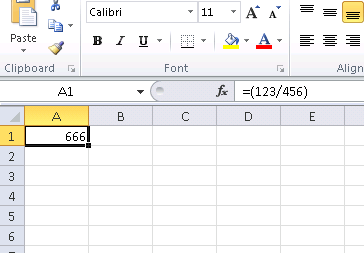
\includegraphics[scale=\NormalScale]{digging_into_code/Excel_prank.png}
\caption{\RU{Пранк сработал}\EN{The practical joke worked}}
\end{figure}

\RU{Если попробовать ту же версию Excel, только x64, то окажется что там инструкций \FDIV всего 12, 
причем нужная нам\EMDASH{}третья по счету.}
\EN{If we try the same Excel version, but in x64,
we will find only 12 \FDIV instructions there,
and the one we looking for is the third one.}

\begin{lstlisting}
tracer.exe -l:excel.exe bpx=excel.exe!BASE+0x1B7FCC,set(st0,666)
\end{lstlisting}

\myindex{x86!\Instructions!DIVSD}
\RU{Видимо, все дело в том, что много операций деления переменных типов \Tfloat и \Tdouble 
компилятор заменил на SSE-инструкции вроде \TT{DIVSD}, 
коих здесь теперь действительно много (\TT{DIVSD} присутствует в количестве 268 инструкций).}
\EN{It seems that a lot of division operations of \Tfloat and \Tdouble types, were replaced by the compiler with SSE instructions
like \TT{DIVSD} (\TT{DIVSD} is present 268 times in total).}

\chapter{\IFRU{Подозрительные паттерны кода}{Suspicious code patterns}}

\section{\IFRU{Инструкции XOR}{XOR instructions}}
\index{x86!\Instructions!XOR}

\IFRU{Инструкции вроде}{instructions like} \TT{XOR op, op} (\IFRU{например}{for example}, \TT{XOR EAX, EAX}) 
\IFRU{обычно используются для обнуления регистра,
однако, если операнды разные, то применяется операция именно}{are usually used for setting register value
to zero, but if operands are different,} \IT{\IFRU{исключающего или}{exclusive or}}\EN{ operation
is executed}.
\IFRU{Эта операция очень редко применяется в обычном программировании, но применяется очень часто в криптографии,
включая любительскую}{This operation is rare in common programming, but used often in cryptography,
including amateur}.
\IFRU{Особенно подозрительно, если второй операнд это большое число}{Especially suspicious case if the
second operand is big number}.
\IFRU{Это может указывать на шифрование, вычисление контрольной суммы, итд}
{This may points to encrypting/decrypting, checksum computing, etc}.\\
\\
\IFRU{Одно из исключений из этого наблюдения о котором стоит сказать, то, что генерация и проверка значения ``канарейки''
(\ref{subsec:BO_protection}) часто происходит используя инструкцию \XOR}
{One exception to this observation worth to note is ``canary'' (\ref{subsec:BO_protection}) generation and checking is often done using \XOR
instruction}. \\
\\
\index{AWK}
\IFRU{Этот AWK-скрипт можно использовать для обработки листингов (.lst) созданных \IDA{}}
{This AWK script can be used for processing \IDA{} listing (.lst) files}:

\begin{lstlisting}
gawk -e '$2=="xor" { tmp=substr($3, 0, length($3)-1); if (tmp!=$4) if($4!="esp") if ($4!="ebp") { print $1, $2, tmp, ",", $4 } }' filename.lst
\end{lstlisting}

\IFRU{Нельзя также забывать,
что если использовать подобный скрипт, то, возможно, он захватит и неверно дизассемблированный
код}{It is also worth to note that such script may also capture incorrectly disassembled code} 
(\ref{sec:incorrectly_disasmed_code}).

\section{\IFRU{Вручную написанный код на ассемблере}{Hand-written assembly code}}

\index{Function prologue}
\index{Function epilogue}
\index{x86!\Instructions!LOOP}
\index{x86!\Instructions!RCL}
\IFRU{Современные компиляторы не генерируют инструкции \TT{LOOP} и \TT{RCL}. 
С другой стороны, эти инструкции хорошо знакомы кодерам, предпочитающим писать прямо на ассемблере. 
Подобные инструкции отмечены как (M) в списке инструкций в приложении: \ref{sec:x86_instructions}.
Если такие инструкции встретились, можно сказать с какой-то вероятностью, что этот фрагмент кода написан вручную.}
{Modern compilers do not emit \TT{LOOP} and \TT{RCL} instructions.
On the other hand, these instructions are well-known to coders who like to code in straight assembly language.
If you spot these, it can be said, with a high probability, this fragment of code is hand-written.
Such instructions are marked as (M) in the instructions list in appendix: \ref{sec:x86_instructions}.}\\
\\
\IFRU{Также, пролог/эпилог функции обычно не встречается в ассемблерном коде, написанном вручную.}
{Also function prologue/epilogue is not commonly present in hand-written assembly copy.}\\
\\
\IFRU{Как правило, в вручную написанном коде, нет никакого четкого метода передачи аргументов в 
функцию}
{Commonly there is no fixed system in passing arguments into functions in the hand-written
code}.\\
\\
\IFRU{Пример из ядра}{Example from} Windows 2003\EN{ kernel} 
(\RU{файл }ntoskrnl.exe\EN{ file}):

\begin{lstlisting}
MultiplyTest proc near               ; CODE XREF: Get386Stepping
             xor     cx, cx
loc_620555:                          ; CODE XREF: MultiplyTest+E
             push    cx
             call    Multiply
             pop     cx
             jb      short locret_620563
             loop    loc_620555
             clc
locret_620563:                       ; CODE XREF: MultiplyTest+C
             retn
MultiplyTest endp

Multiply     proc near               ; CODE XREF: MultiplyTest+5
             mov     ecx, 81h
             mov     eax, 417A000h
             mul     ecx
             cmp     edx, 2
             stc
             jnz     short locret_62057F
             cmp     eax, 0FE7A000h
             stc
             jnz     short locret_62057F
             clc
locret_62057F:                       ; CODE XREF: Multiply+10
                                     ; Multiply+18
             retn
Multiply     endp
\end{lstlisting}

\IFRU{Действительно, если заглянуть в исходные коды}{Indeed, if we look into} 
\ac{WRK} v1.2\IFRU{, данный код можно найти в файле}{ source code, this code
can be found easily in the file} 
\IT{WRK-v1.2\textbackslash{}base\textbackslash{}ntos\textbackslash{}ke\textbackslash{}i386\textbackslash{}cpu.asm}.

\section{\IFRU{Использование magic numbers для трассировки}{Using magic numbers while tracing}}

\IFRU{Нередко бывает нужно узнать, как используется то или иное значение прочитанное из файла либо взятое из пакета
принятого по сети. Часто, ручное слежение за нужной переменной это трудный процесс. Один из простых методов (хотя и не
полностью надежный на 100\%) это использование вашей собственной \IT{magic number}.}
{Often, main goal is to get to know, how a value was read from file, or received via network, being used. 
Often, manual tracing of a value is very labouring task. One of the simple methods (however, not 100\% reliable) 
is to use your own \IT{magic number}.}

\IFRU{Это чем-то напоминает компьютерную томографию: пациенту перед сканированием вводят в кровь 
рентгеноконтрастный препарат, хорошо отсвечивающий в рентгеновских лучах. Известно как кровь нормального человека
расходится, например, по почкам, и если в этой крови будет препарат, то при томографии будет хорошо видно,
достаточно ли хорошо кровь расходится по почкам и нет ли там камней, например, и прочих образований.}
{This resembling X-ray computed tomography is some sense: radiocontrast agent is often injected into patient's blood,
which is used for improving visibility of internal structures in X-rays. For example, it is well known how blood of healthy man/woman
percolates in kidneys and if agent is in blood, it will be easily seen on tomography, how good and normal blood was percolating,
are there any stones or tumors.}

\IFRU{Мы можем взять 32-битное число вроде \IT{0x0badf00d}, либо чью-то дату рождения вроде \IT{0x11101979} 
и записать это, занимающее 4 байта число, в какое-либо место файла используемого исследуемой нами программой.}
{We can take a 32-bit number like \IT{0x0badf00d}, or someone's birth date like \IT{0x11101979}
and to write this, 4 byte holding number, to some point in file used by the program we investigate.}

\index{\GrepUsage}
\IFRU{Затем, при трассировки этой программы, в том числе, при помощи \tracer в режиме 
\IT{code coverage}, а затем при помощи
\IT{grep} или простого поиска по текстовому файлу с результатами трассировки, мы можем легко увидеть, в каких местах кода использовалось 
это значение, и как.}
{Then, while tracing this program, with \tracer in the \IT{code coverage} mode, and then, with the help of \IT{grep}
or just by searching in the text file (of tracing results), we can easily see, where the value was used and how.}

\IFRU{Пример результата работы \tracer в режиме \IT{cc}, к которому легко применить утилиту \IT{grep}}{Example 
of \IT{grepable} \tracer results in the \IT{cc} mode}:

\begin{lstlisting}
0x150bf66 (_kziaia+0x14), e=       1 [MOV EBX, [EBP+8]] [EBP+8]=0xf59c934 
0x150bf69 (_kziaia+0x17), e=       1 [MOV EDX, [69AEB08h]] [69AEB08h]=0 
0x150bf6f (_kziaia+0x1d), e=       1 [FS: MOV EAX, [2Ch]] 
0x150bf75 (_kziaia+0x23), e=       1 [MOV ECX, [EAX+EDX*4]] [EAX+EDX*4]=0xf1ac360 
0x150bf78 (_kziaia+0x26), e=       1 [MOV [EBP-4], ECX] ECX=0xf1ac360 
\end{lstlisting}

\IFRU{Это справедливо также и для сетевых пакетов.
Важно только чтобы наш \IT{magic number} был как можно более уникален и не присутствовал в самом коде.}
{This can be used for network packets as well.
It is important to be unique for \IT{magic number} and not to be present in the program's code.}

\newcommand{\DOSBOXURL}{\url{http://blog.yurichev.com/node/55}}

\index{DosBox}
\IFRU{Помимо \tracer, такой эмулятор MS-DOS как DosBox, в режиме heavydebug, может писать в отчет информацию обо всех
состояниях регистра на каждом шаге исполнения программы\footnote{См.также мой пост в блоге об этой возможности в 
DosBox: \DOSBOXURL{}}, так что этот метод может пригодиться и я для исследования программ под DOS.}{Aside of 
\tracer, DosBox (MS-DOS emulator) in heavydebug mode,
is able to write information about all register's states for each executed instruction of program to plain text file\footnote{See also my 
blog post about this DosBox feature: \DOSBOXURL{}}, so this method may be useful for DOS programs as well.}



\chapter{\RU{Прочее}\EN{Other things}}

\section{\EN{General idea}\RU{Общая идея}}

\RU{Нужно стараться как можно чаще ставить себя на место программиста и задавать себе вопрос, 
как бы вы сделали ту или иную вещь в этом случае и в этой программе.}
\EN{A reverse engineer should try to be in programmer's shoes as often as possible. 
To take his/her viewpoint and ask himself, how would one solve some task the specific case.}

\section{\Cpp}

\ac{RTTI}~(\myref{RTTI})-\RU{информация также может быть полезна для идентификации 
классов в \Cpp}\EN{data may be also useful for \Cpp class identification}.

\section{\RU{Некоторые паттерны в бинарных файлах}\EN{Some binary file patterns}}
\index{MIPS}

\EN{Sometimes, we can clearly spot an array of 16/32/64-bit values visually, in hex editor.}
\RU{Иногда мы можем легко заметить массив 16/32/64-битных значений визуально, в шестнадцатеричном 
редакторе.}
\EN{Here is an example of very typical MIPS code.}
\RU{Вот пример очень типичного MIPS-кода.}
\EN{As we may remember, every MIPS (and also ARM in ARM mode or ARM64) instruction has size of 32 bits (or 4 bytes), 
so such code is array of 32-bit values.}
\RU{Как мы наверное помним, каждая инструкция в MIPS (а также в ARM в режиме ARM, или ARM64) имеет 
длину 32 бита (или 4 байта),
так что такой код это массив 32-битных значений.}
\EN{By looking at this screenshot, we may see some kind of pattern.}
\RU{Глядя на этот скриншот, можно увидеть некий узор.}
\EN{I added vertical red lines for clarity}\RU{Я добавил вертикальные красные линии для ясности}:

\begin{figure}[H]
\centering
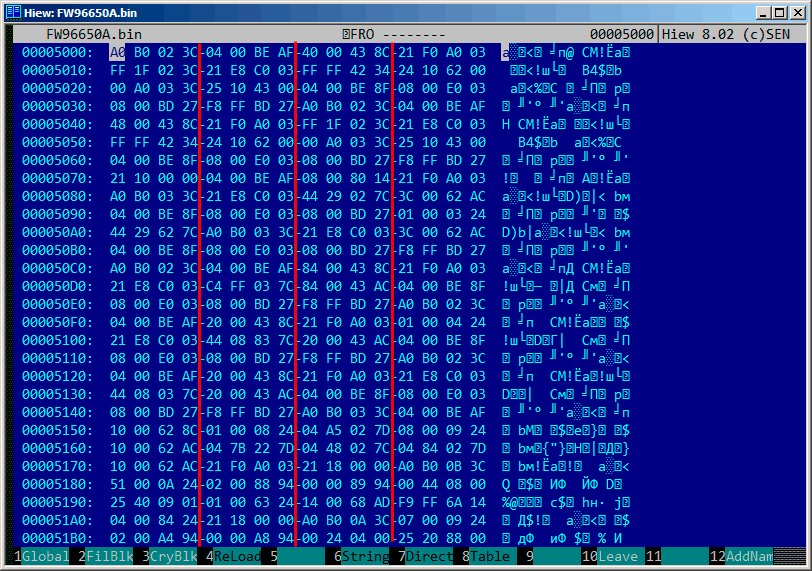
\includegraphics[scale=\NormalScale]{digging_into_code/typical_MIPS_code.png}
\caption{Hiew: \EN{very typical MIPS code}\RU{очень типичный код для MIPS}}
\end{figure}

\RU{Еще пример таких файлов в этой книге}\EN{Another example of such pattern here is book}: 
\myref{Oracle_SYM_files_example}.

\subsection{\IFRU{Сравнение ``снимков'' памяти}{Memory ``snapshots'' comparing}}

\IFRU{Метод простого сравнения двух снимков памяти для поиска изменений часто применялся для взлома игр 
на 8-битных компьютерах и взлома файлов с записанными рекордными очками.}
{The method of simple two memory snapshots comparing in order to see changes, was often used to hack
8-bit computer games and hacking ``high score'' files.}

\IFRU{К примеру, если вы имеете загруженную игру на 8-битном компьютере (где самой памяти не очень много, но игра
занимает еще меньше), и вы знаете что сейчас у вас, условно, 100 пуль, вы можете сделать ``снимок'' всей
памяти и сохранить где-то. Затем просто стреляете куда угодно, у вас станет 99 пуль, сделать второй ``снимок'',
и затем сравнить эти два снимка: где-то наверняка должен быть байт, который в начале был 100, а затем стал 99.}
{For example, if you got some loaded game on 8-bit computer (it's not much memory on these, but game is usually
consumes even less memory) and you know that you have now, let's say, 100 bullets, you can do a ``snapshot''
of all memory and save it to some place. Then shoot somewhere, bullet count now 99, do second ``snapshot''
and then compare both: somewhere should be a byte which was 100 in the beginning and now it's 99.}
\IFRU{Если учесть что игры на тех маломощных домашних компьютерах обычно были написанны на ассемблере и подобные
переменные там были глобальные, то можно с уверенностью сказать, какой адрес в памяти всегда отвечает за количество
пуль. Если поискать в дизассемблированном коде игры все обращения по этому адресу, несложно найти код,
отвечающий за уменьшение пуль и записать туда инструкцию \NOP\footnote{``no operation'', холостая инструкция} 
или несколько \NOP-в, так мы получим игру в которой у игрока всегда будет 100 пуль, например.}
{Considering a fact that these 8-bit games were often written in assembler and such variables were global,
it can be said for sure, which address in memory holding bullets count. If to search all references to that
address in disassembled game code, it's not very hard to find a piece of code decrementing bullets count,
write \NOP instruction\footnote{``no operation'', idle operation} there, or couple of \NOP{}-s, 
we'll have a game with 100 (for example) bullets forever.}
\IFRU{А так как игры на тех домашних 8-битных 
компьютерах всегда загружались по одним и тем же адресам, и версий одной игры редко когда было больше одной,
то геймеры-энтузиасты знали, по какому адресу (используя инструкцию языка BASIC \IT{POKE}\footnote{инструкция языка BASIC записывающая байт по определенному адресу}) что записать после загрузки
игры, чтобы хакнуть её. Это привело к появлению списков ``читов'' состоящих из инструкций \IT{POKE}, публикуемых
в журналах посвященным 8-битным играм. См.также:}{Games on these 8-bit computers was usually loaded on the same
address, also, there were no much different versions of each game (usually, just one version all have),
enthusiastic gamers knew, which byte should be written (using BASIC instruction \IT{POKE}\footnote{BASIC language instruction writting byte on specific address}) to which address in
order to hack it. This led to ``cheat'' lists containing of \IT{POKE} instructions published in magazines related to
8-bit games. See also:} \url{http://en.wikipedia.org/wiki/PEEK\_and\_POKE}.

\IFRU{Точно также легко модифицировать файлы с сохраненными рекордами, кто сколько очков набрал, впрочем, это может
сработать не только с 8-битными играми. Нужно заметить, какой у вас сейчас рекорд и где-то сохранить файл
с очками. Затем, когда очков станет другое количество, просто сравнить два файла, можно даже
DOS-утилитой FC\footnote{утилита MS-DOS для сравнения двух файлов побайтово} (файлы рекордов, часто, бинарные).}
{The same story about modifying ``high score'' files, this may work not only with 8-bit games. Let's notice 
your score count and save the file somewhere. When ``high score'' count will be different, just compare two files,
it can be even done with DOS-utility FC\footnote{MS-DOS utility for binary files comparing} (``high score'' files
are often in binary form).}
\IFRU{Где-то будут отличаться несколько байт, и легко будет увидеть, какие именно отвечают за количество очков. 
Впрочем, разработчики игр осведомлены о таких хитростях и могут защититься от этого.}
{There will be some place where couple of bytes will be different and it will be easy to see which ones are
holding score number.
However, game developers are aware of such tricks and may protect against it.}

% FIXME: пример с какой-то простой игрушкой?


